\documentclass[]{report}
\usepackage[]{fbb}
\usepackage[top=45mm, bottom=45mm, left=25mm, right=25mm]{geometry}
\usepackage{tikz}
\usetikzlibrary{positioning, shapes.geometric, arrows}

\tikzset{
	block/.style={
		rectangle,
		draw,
		text width=1cm,
		text centered,
		minimum height=1cm,
		rounded corners=5pt,
		fill=black!10,
	},
	sum/.style={
		circle,
		draw,
		text centered,
		fill=black!10,
		inner sep=0pt,
		minimum size=0.6cm,
	},
	delay/.style={
		draw,
		shape=isosceles triangle,
		shape border rotate=0,
		inner sep=0pt,
		minimum height=1cm,
		fill=black!10,
	},
}

\title{\textbf{Lab Report Title}}
\date{\textit{\today}}
\author{Arnav Goyal - 251244778}

\begin{document}
	\maketitle
	\section*{Algorithms}
	Here are the three methods (algortihms) presented in the lab report
	
	\begin{equation}
		v_{avg}(n) = \frac{1}{4} \left(  v(n) + v(n-1) + v(n-2) + v(n-3) \right)
	\end{equation}
	
	\begin{equation}
		v_{avg}(n) = 0.3 \cdot v(n) + 0.7 \cdot v_{avg}(n-1)
	\end{equation}
	
	\begin{equation}
		v_{avg}(n) = \frac{1}{4} \left( v(n) - v(n-4)  \right) + v_{avg}(n-1)
	\end{equation}
	
	\section*{Block Diagrams}

	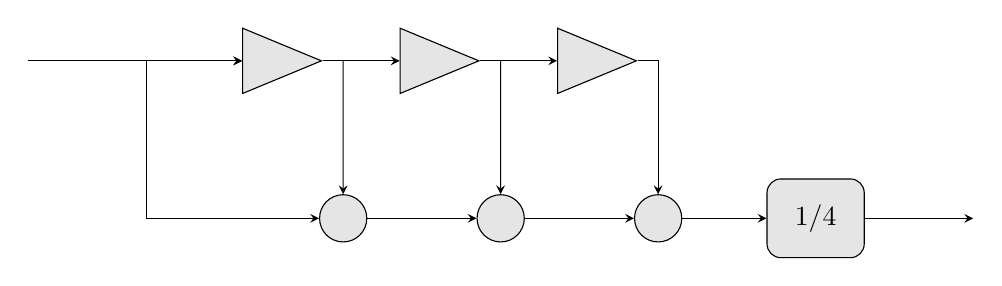
\begin{tikzpicture}[node distance = 2cm , >=stealth]
		% Place nodes
		\node [delay] (d1) {};
		\node [delay, right of = d1] (d2) {};
		\node [delay, right of = d2] (d3) {};
		
		\draw [->] (d1)++(-1.5,0) to (d1);
		\draw [->] (d1) to (d2);
		\draw [->] (d2) to (d3);
		
		\node[sum, below of = d1, xshift=1cm] (s1) {};
		\node[sum, below of = d2, xshift=1cm] (s2) {};
		\node[sum, below of = d3, xshift=1cm] (s3) {};
		
		\draw [->] (d1)++(-1.5,0) |- (s1);
		\draw [->] (d2)++(-1,0) to (s1);
		
		\draw [->] (s1) to (s2);
		\draw [->] (d3)++(-1,0) to (s2);
		
		\draw [->] (s2) to (s3);
		\draw [->] (d3) -| (s3);
		
		\node [block, right of = s3] (fac) {1/4};
		
		\draw [->] (s3) to (fac);
		\draw [->] (fac) to ++(2,0);
		\draw [->] (d1)++(-3,0) to (d1);

	\end{tikzpicture}
	
\end{document}
